\subsubsection{UC4 - Salvataggio credenziali su file}
\begin{figure}[h]
	\centering
	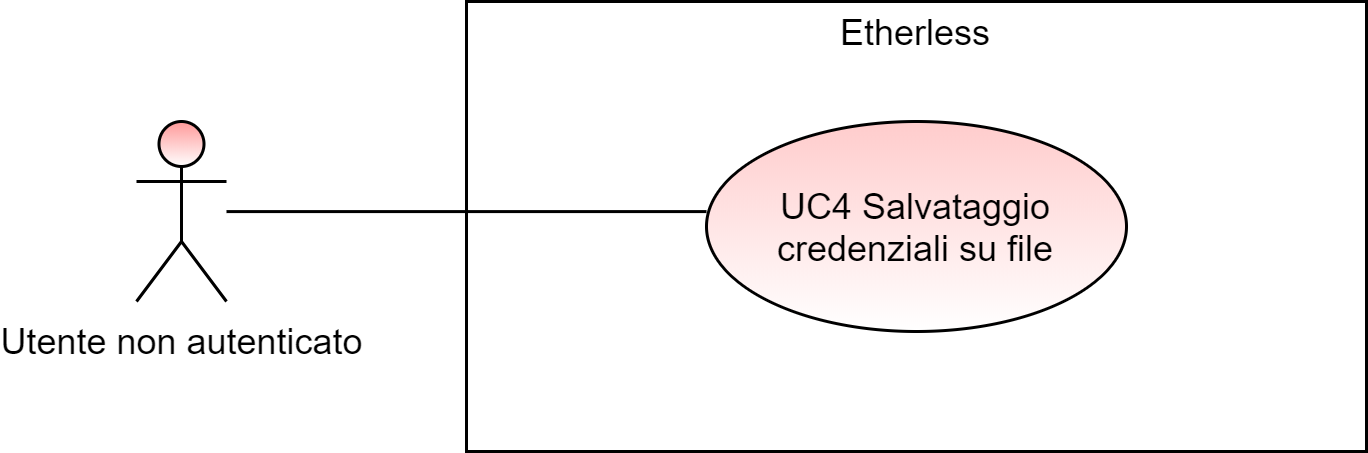
\includegraphics[scale=\ucs]{./res/img/UC4G.png}
	\caption {UC4 - Salvataggio credenziali su file: schema generale}
\end{figure}
\begin{itemize}
	\item \textbf{Attori primari:} \una{};
	\item \textbf{Descrizione:} a seguito della creazione di una nuova utenza Ethereum l’utente può richiedere al sistema il salvataggio su file delle credenziali dell’account creato. Tali credenziali includono address, private key e mnemonic phrase.
	\item \textbf{Scenario principale:}
	\begin{itemize}
		\item l’utente richiede di salvare su file le informazioni del nuovo account creato; 
		\item il sistema si occupa del corretto salvataggio delle credenziali. 
	\end{itemize}
	\item \textbf{Precondizione:} l’utente richiede di salvare le informazioni relative al nuovo account tramite l’utilizzo del flag \texttt{-s};  
	\item \textbf{Postcondizione:} le credenziali sono state salvate con successo all’interno del file.  
\end{itemize}